% RUN in terminal (without bibliography):
% pdflatex -output-directory=/Users/salvatorpes/Desktop/LFEUI/text/proposta /Users/salvatorpes/Desktop/LFEUI/text/proposta/prop.tex

\documentclass{article}

\author{
    \begin{tabular}{rl}
        Estêvão Gomes (ist1102650) & Sofia Nunes (ist1102633) \\
        Pedro Curvo (ist1102716) & Salvador Torpes (ist1102474)
    \end{tabular}
}

\usepackage[utf8]{inputenc}
\usepackage[english]{babel}
\usepackage[letterpaper,top=6mm,bottom=15mm,left=6mm,right=6mm,marginparwidth=1.55cm]{geometry}
\usepackage{multicol}
\usepackage{graphicx}
\usepackage{subcaption}
\usepackage{tabularx}
\usepackage{booktabs}
\usepackage{array}
\usepackage{makecell}
\usepackage{titlesec}
\usepackage{multirow}
\usepackage{amsmath}
\usepackage{makecell}
\usepackage{url}
\usepackage{csquotes}
\usepackage{caption}
\usepackage{enumitem}
\usepackage{textcomp}
\usepackage{pdflscape}
\usepackage{makeidx}
\usepackage{mathtools}
% \usepackage{tocbibind}
\providecommand{\tightlist}{\relax}
\usepackage{tocloft}
\renewcommand{\cftsecindent}{0em}
\renewcommand{\cftsubsecindent}{1em}
\renewcommand{\cftsecfont}{\bfseries}
\renewcommand{\cftsubsecfont}{\itshape}
\setlength{\cftsubsecnumwidth}{0em}

\usepackage[version=4]{mhchem}
\usepackage{hyperref} % Remove "pdftex" option here
\usepackage{float}
\usepackage{fancyhdr}
\usepackage{ragged2e}
\usepackage{xkeyval}
%\usepackage{minted}
%\usemintedstyle{manni}
\usepackage{listings}
\usepackage{amssymb}


\usepackage{xcolor}
\usepackage{tikz}

\usetikzlibrary{positioning}
\usetikzlibrary{positioning, arrows.meta}
\usepackage{adjustbox}
\usepackage{sidecap}
\usepackage{graphicx}

\usepackage{tikz-3dplot}
\usepackage{pgfplots}
\usetikzlibrary{calc, 3d, arrows}



\usetikzlibrary{shapes.geometric, arrows}


\lstset{
    language=Python,
    basicstyle=\ttfamily,
    keywordstyle=\color{blue},
    commentstyle=\color{gray},
    stringstyle=\color{orange},
    numbers=left,
    numberstyle=\tiny,
    numbersep=5pt,
    showspaces=false,
    showstringspaces=false,
    breaklines=true,
    frame=tb,
    framexleftmargin=2em,
    xleftmargin=2em,
}


%\usepackage{fontspec}

%\setmonofont{Fira Code}

\fancyhf{}
\cfoot{\thepage}
\fancyhf{} % Clear all header and footer fields
\renewcommand{\headrulewidth}{0pt} % Remove the header rule line
\cfoot{\thepage} % Set the page number in the center of the footer

\pagestyle{fancy} % Apply the fancy page style

\setlength\columnsep{20pt}

\renewcommand{\familydefault}{\sfdefault}

\newenvironment{Figure}
  {\par\medskip\noindent\minipage{\linewidth}}
  {\endminipage\par\medskip}

\makeatletter
\newenvironment{figurehere}
{\def\@captype{figure}}
{}
\makeatother

\hypersetup{
  colorlinks,
  linkcolor=blue,
  anchorcolor=black,
  citecolor=cyan,
  filecolor=cyan,
  menucolor=cyan,
  urlcolor=cyan,
  bookmarksopen=true,
  bookmarksnumbered=true
}

\makeindex


\title{\vspace{-13mm}
\includegraphics[width=15mm,scale=3]{../images/IST_Logo.png}
% \\ \vspace{1mm} LFEUI \vspace{1mm} 
\\ {\fontsize{24}{16}Detection of Li in Technological Materials through Nuclear Reactions} \vspace{-5mm}}
\date{December 2023 - January 2024}

\usepackage{sansmathfonts}
\usepackage[T1]{fontenc}
\usepackage[OT1]{fontenc}

\titleformat{\section}{\normalfont\large\bfseries}{\thesection}{1em}{}



\usepackage[style=numeric]{biblatex} % Choose your desired citation style
\addbibresource{../references/prop.bib} % Specify your .bib file

\setlist[enumerate]{itemsep=3pt}

\begin{document}

\renewcommand{\arraystretch}{1.5}
\setlength{\columnseprule}{0.4pt}
\tdplotsetmaincoords{70}{110} % Set the viewing angle
\newcolumntype{M}[1]{>{\centering\arraybackslash\vspace{#1}}m{0.5\linewidth}<{\vspace{#1}}}
\newcolumntype{C}[2]{>{\centering\arraybackslash\vspace{#1}\rule{0pt}{#1}\hspace{0pt}}m{#2}}
\newcolumntype{w}[1]{>{\centering\arraybackslash}m{#1}}

\renewcommand*\familydefault{\sfdefault} %% Only if the base font of the document is to be sans serif

\maketitle

\vspace{-8mm}


\hrulefill

% \begin{center}
%   \textbf{\Large Abstract}
% \end{center}

\vspace{-0.1cm}
\begin{abstract}
  \par 
\end{abstract}
\vspace{-0.1cm}

\hrulefill


\begin{multicols}{2}

\section{Main Goal}
    \label{sec:maingoal}

Our main goal is to develop a scientific research project alongside three senior investigators from CTN (Centro Tecnológico e Nuclear), Rodrigo Mateus, Rui Silva and Norberto Catarino.
Our project will be focused on the detection of Li in technological materials through nuclear reactions. The main motivation for this project is to study and develop a detection technique for elements such as Li with high sensitivity. 

\section{Scientific Background}
    \label{sec:scientificbackground}

The development of this scientific procedure is based on a physics phenomenon: nuclear reactions. We have an accelerator in order to allow protons with specific energy to collide with the sample whose composition we are interested in studying. The protons will undergo a nuclear reaction with the ones in the samples and byproducts of these reaction will be released. These byproducts are charged particles and we can detect their energy spectrum. Through the analysis of it, we want to infer what were the elements with whom they reacted on the sample and what is their composition percentage.

\subsection{Nuclear Reaction}
    \label{sec:nuclearreactions}

The main nuclear reaction in which we are interested is the one between $\ce{^7Li}$ and an incoming proton on the beam:

\begin{equation}
  \ce{^7Li + ^1H -> ^8Be -> 2\alpha}
\label{eq:reactionLi}
\end{equation}

Before the emission of the reaction products, the reaction leads to the formation of a $\ce{^8Be}$ compound nucleus (intermediate state), which then rapidly decays into two alpha particles. These are the particles we detect. An alpha particle is a helium nucleus, composed of two protons and two neutrons.

\paragraph{} Some of the samples we are going to work with also include boron and according to the beam energy we use it is possible that the protons lead to a nuclear reaction with the boron atoms in the samples. Therefore, the $\ce{^{11}B}$ reaction with a proton is as follows:

\begin{equation}
  \ce{ ^{11}B + ^1H -> ^{12}C -> ^8Be + \alpha}
\label{eq:reactionB}
\end{equation}

The reaction first leads to the formation of a $\ce{^{12}C}$ compound nucleus which decays into one alpha particle and a $\ce{^8Be}$ nucleus. The $\alpha$ particle can be detected with more or less energy according to the energy level on which the $\ce{^8Be}$ nucleus is emitted. If the latter is on the fundamental state, the $\alpha$ particle will have more energy and if it is on a higher state, the $\alpha$ particle will have less energy.

\subsection{Energy Peaks and Energy Profile}
    \label{sec:energy_profile_peak}

In what comes to the phenomena we expect to see in the collected energy spectrum's, the first one are the energy values themselves. Both the alpha particles and the other byproducts are emitted with a specific energy just after the nuclear reaction, and this energy can be computed according to the reaction itself and also to the beam's energy. This calculus will be done in section \ref{sec:theoreticalvalues}. 
\paragraph{}
Firstly, we expect to see intensity peaks on the spectrum on these specific energies. However, we must take into account the fact that before arriving at the detector, the emitted particles have to go through the other atoms on the sample. As an incident proton comes in, it might react with another proton from the material that sits on its surface but it can also react with one inside it. The byproducts produced inside the sample initially have the energy we compute but do lose part of it as they collide with other particles before reaching the detector. Basically, we must consider the sample's thickness. The bigger the depth at which the reaction takes place, the smaller the energy with whom they are detected because more of it gets dissipated.
Therefore, this will result in an energy profile - the energy peak will be gradually preceded by less intense peaks due to particles that lost energy on their way to the detector. It is less likely for the particles that are emitted inside the sample to reach the detector than for those who were emitted on its surface since on each collision there is a chance that it's direction might change. This is why the intensity on the energy profile as a steady increase before hitting a maximum value at the energy with whom the particle comes out of the reaction
\paragraph{}
We expect this phenomena to be particularly significant in samples where the atom that takes part in the reaction can be found not only at the surface of the sample but also in its depth. Therefore, in implanted samples where the substrate is only a layer, the energy profile will be less evident.

\subsection{Elastic Back-scattering}

One other feature that might occur is elastic back-scattering. This happens when the incoming proton from the accelerator is elastically reflected by the sample and then detected. After the reflection, the energy is the same and this means that there will be an intensity peak located at the selected beam energy.

\subsection{Rutherford Back scattering}

Rutherford back-scattering is a phenomena that occurs when the incoming proton is reflected by the sample but, in this case, the energy is not the same. This means that the proton loses energy on the reflection and therefore the intensity peak will be located at a lower energy than the selected beam energy.

\section{Experimental Procedure}
    \label{sec:experimentalprocedure}

\subsection{Work Plan}
    \label{sec:workplan}

Obtaining the energy spectrum of the particles resulting from the nuclear reactions between the protons and the samples will take the following steps:

\begin{enumerate}
  \item Accelerator Startup - beam energy increase;
  \item Sample Preparation;
  \item Channel-energy calibration of the detection system with a well-known triple $\alpha$ source;
  \item Lenses and electromagnets set up and adjustment;
  \item Obtaining the energy spectrum of all samples;
\end{enumerate}

\subsection{Experimental Set-Up}
    \label{sec:setup}

The experimental set-up consists of a Tandem accelerator, a beam line with electromagnets and a chamber with both the samples and the detectors. 

Theoretically, the accelerator produces a beam of protons with a kinetic energy of up to 5 MeV, which is deviated by the steering electromagnet before hitting the sample. The electromagnet deflect particles with different angles according to their charge-to-mass ratio and, with that, allows us to remove any unwanted particles from the beam and only let the protons pass through. 

The detectors used, which are silicon-based, detect charged particles through the ionisation they produce in the silicon.

In addition, the detectors are connected to a electronic system that amplifies the signal and sends it to a computer where the spectra can be seen.

The beam line is under a vacuum of around $10^{-7}$ mbar in order to avoid the protons colliding with other particles and losing energy. They reach the sample with the specified kinetic energy and cause a nuclear reaction whose products are the charged particles detected. We aim to analyse the energy spectrum of these particles.

\begin{center}
    \label{TT_21}
    \centering
    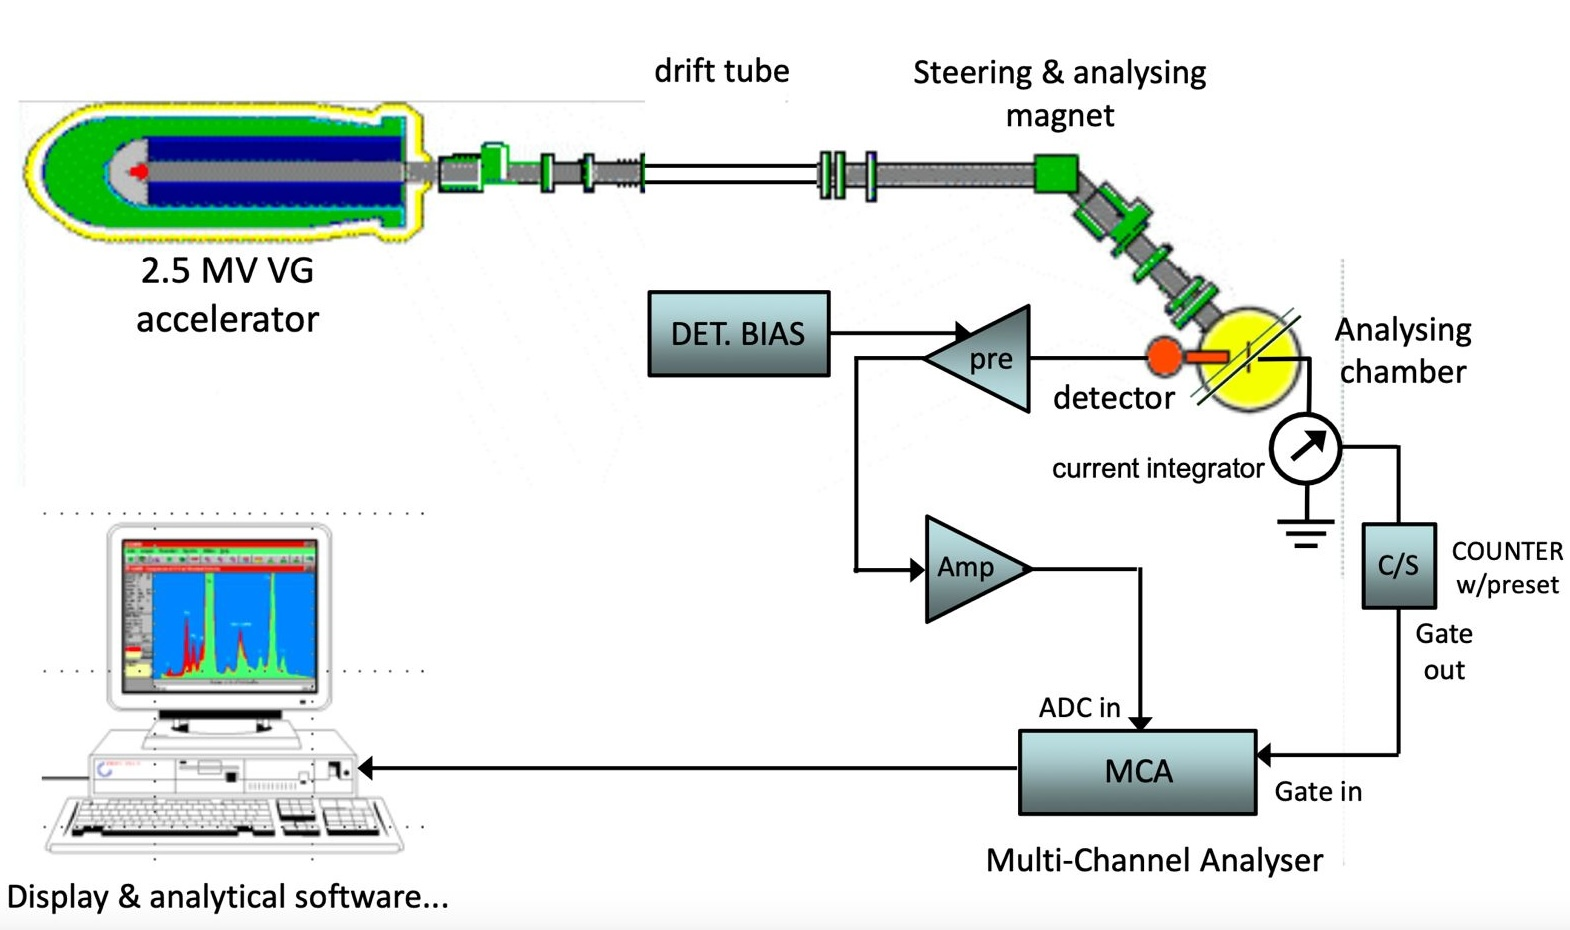
\includegraphics[scale = 0.15]{images/scheme.jpeg}
    \captionof{figure}{Experimental Set-up}
\end{center}

\subsection{Beam Energy Selection}
    \label{sec:beamenergyselection}

In order to choose the energy of the beam we need to take into account the cross section of the reaction between the protons and the Li-7. We collected data from the IBANDL database for this reaction in a range of [0.5,7] MeV and plotted it in the following graph:

\begin{center}
    \label{TT_21}
    \centering
    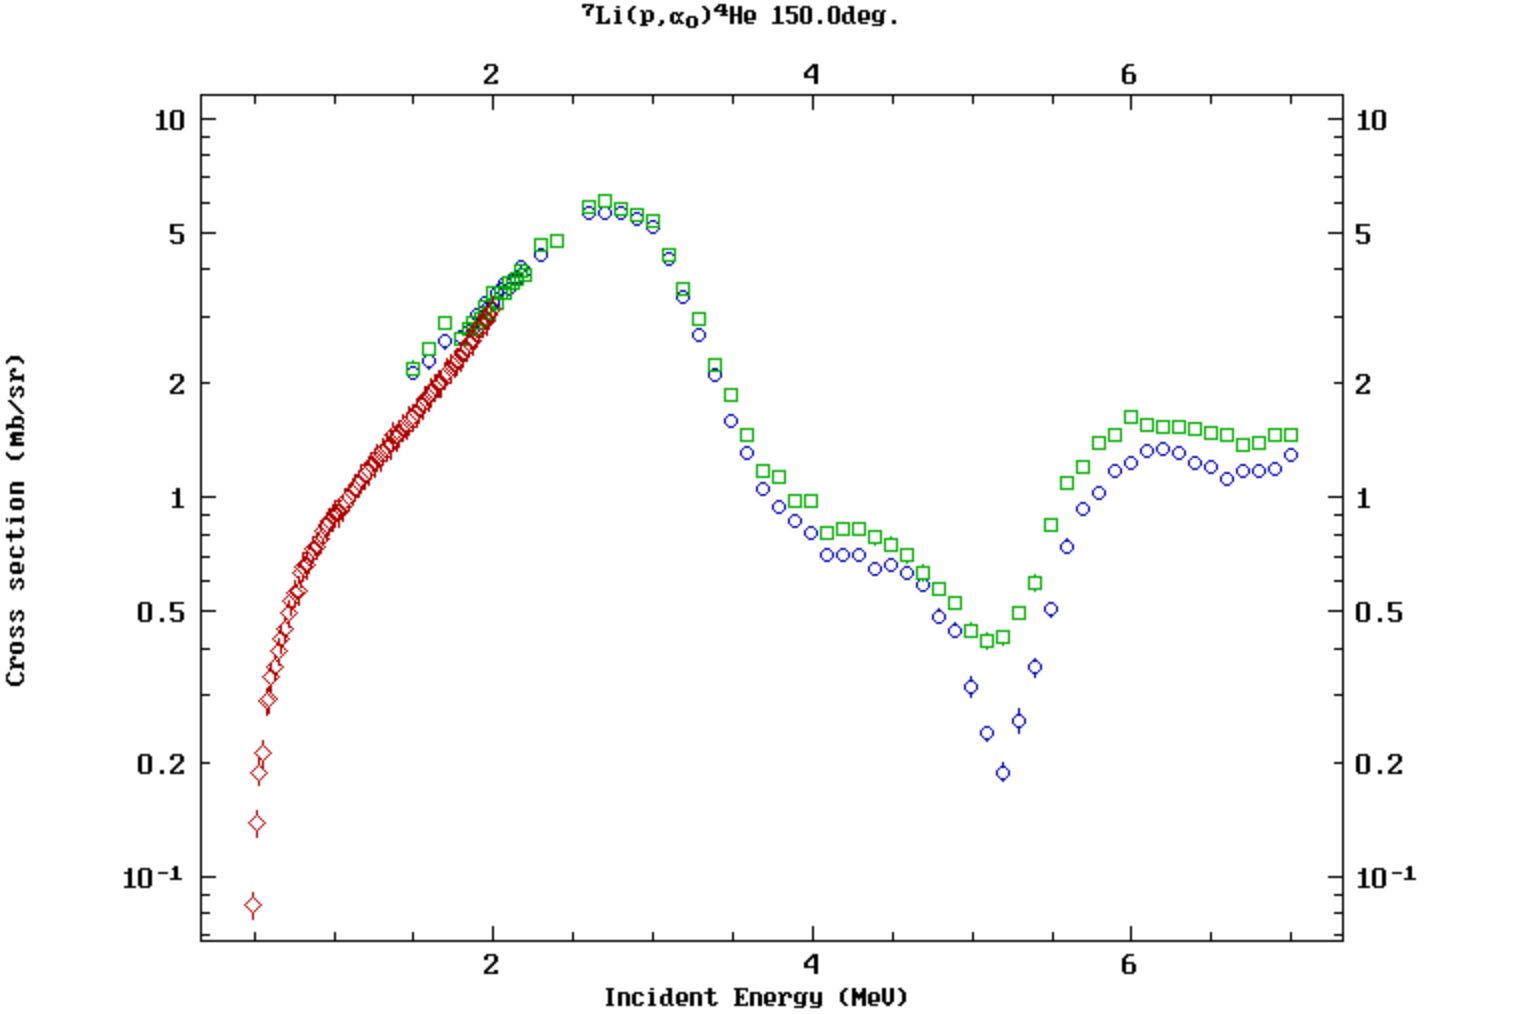
\includegraphics[scale = 0.17]{images/Li_crosssection_energy.jpeg}
    \captionof{figure}{Cross section of the reaction between protons and Li-7 as a function of the beam energy}
\end{center}

We are only interested in the energy range of [0.5,5] MeV because the energy of the beam is limited by the accelerators range. As we can see in the above figure, the cross section of the reaction is maximum in the [2.5, 3] MeV range. Therefore, since we want to detect the Li-7 in the samples, we should choose the energy of the beam to be in this range. 
\paragraph{}
However, practically, the accelerator cannot reach a beam within the [2.5, 3] MeV energy range. Increasing beam energies take exponentially more time to be set up. Also, we are interested in the possible boron identification in some of the used samples. Boron does not react with such high energies but a lower energy beam is effective in doing that.
Having this into consideration, we choose a beam energy of $1.3$ MeV for our experimental procedure.

\subsection{NRA Calculations - Theoretical Values}
    \label{sec:theoreticalvalues}

After concluding that the best beam energy to work within the previously described conditions is $1.3$ MeV, we now need to obtain theoretical values for their energy. In order to do this, we will use the NRA calculator \cite{NRAEnergyCalc}. This is an online calculator developed by investigators at CTN that allows researchers to compute the $Q$ value of a reaction as well as the energy values and scattering angles of the particles these reactions emit. Considering an incident beam whose protons have $E_p = 1.3$ MeV and a scattering angle of $\theta = 165 ^{\circ}$ of our detector we computed the following values:

\paragraph{Lithium} Firstly, for the reaction \ref{eq:reactionLi}:

\begin{equation}
\begin{split}
  E_{\alpha_{0_1}} &= 7.6298 \text{ MeV} \\
  E_{\alpha_{0_2}} &= 11.0314 \text{ MeV} \\
  \theta_{\alpha_{0_1}} &= 165 ^{\circ} \\
  \theta_{\alpha_{0_2}} &= 12 ^{\circ} \\
  Q (\ce{^7Li}) &= 17.346 \text{ MeV} \\
\end{split}
\label{eq:energiesli}
\end{equation}

$E_{\alpha_{0_1}}$ and $E_{\alpha_{0_2}}$ are the energies of both alpha particles considering that they are in the fundamental state. In this case, the only other option would be for the $\ce{^8Be}$ to be formed in an excited state and therefore give origin to alpha particles also in an excited state. There is not enough energy for this to happen since the difference between the ground state and the the first state in an helium nuclei is very big, around $INSERT$ MeV.
\paragraph{}
Also, we can see that the scattering angle of the second alpha particle is around $12 ^{\circ}$ meaning that it is different from the detector's angle and will not be detected. To sum up, if there is lithium in any sample that reacts with the incoming protons according to \ref{eq:reactionLi}, we expect to detect alpha particles that were emitted with $7.6298 \text{ MeV}$. 

\paragraph{Boron} Secondly, for the reaction \ref{eq:reactionB}:

\begin{equation}
\begin{split}
  E_{\alpha_0} &= 3.7372 \text{ MeV} \\
  E_{\ce{^8Be}} &= 3.1086 \text{ MeV} \\
  \theta_{\alpha_0} &= 165 ^{\circ} \\
  \theta_{\ce{^8Be}} &= 11 ^{\circ}\\
  Q (\ce{^11Br}) &= 8.591 \text{ MeV} \\
\end{split}
\label{eq:energiesBr}
\end{equation}

We need to comment these energies.

\subsection{Procedure}
    \label{sec:procedure}

We started by displaying the samples in a vertical sample holder with the given order: in the lowest position the implanted sample, followed by lithium aluminate ($\ce{LiAlO2}$) and finally lithium fluoride ($\ce{LiF}$). So that we can do a calibration from the number of counts per channel to energy, we put an additional source on the holder just above the lithium fluoride one. Using a ruler, we measured the distance between the samples so that afterwards we could control the lift in order to change the sample on the beam's target.

We placed the sample holder on a support and afterwards both of them inside the chamber. A vacuum machine was connected to the accelerator to reduce the pressure inside both the chamber and the beam.

Afterwards, we started the procedure to turn on the TANDEM accelerator, according to the provided instruction manual. Firstly, we turned on the $\ce{H^+}$ duoplasmatron source of the accelerator as well as the magnets and lenses. Then, we opened the valves to propagate the vacuum throughout the entirety of the tubes.

In the control panel, we adjusted the angles of the lenses and the magnets current according to the manual, so that the beam would reach the samples. Finally, we used a collimator with a 2mm radius to collimate the beam. 

Finally, we used a computer program to obtain the spectra of the different sources. The multichannel analyzer (MCA) utilized to acquire data was gradually set to 70 V and the angle between the top two detectors was 165º. 

\section*{Analysis}

\section{Calibration}
    \label{sec:calibration}

For the calibration, we used a triple $\alpha$ source. 
In order to do this procedure, for each of spectrum relevant peaks, we need to find the channel with the maximum number of counts.
Then, we find the theoretical values for these peaks and, using both the experimental values for the peaks in channel units and the theoretical ones in MeV, we want to obtain a mathematical relation that allows us to convert channel values into energy values.  
To accomplish this, we will make a linear regression with the energy-channel data. 

The spectrum obtained for the triple source was the following:

\begin{center}
    \label{TT_21}
    \centering
    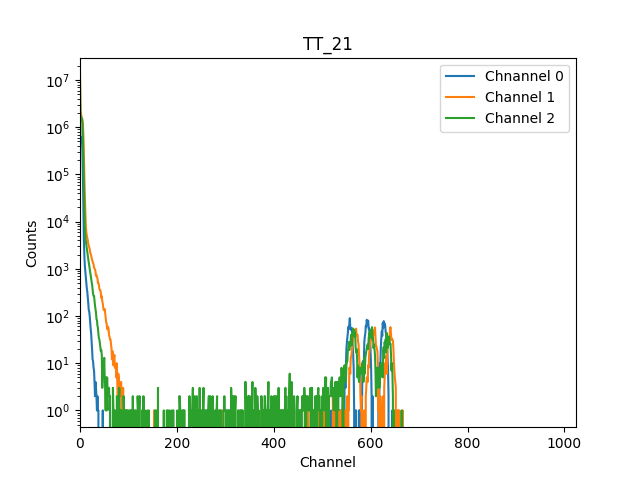
\includegraphics[scale = 0.6]{images/TT_21.png}
    \captionof{figure}{Spectrum of the Calibration source}
\end{center}

We separated the spectra of channels 0, 1 and 2 and used a triple gaussian sum function to fit on the three energy peaks. According to theory, the first peak corresponds to the decay of plutonium into uranium, the second of americium into neptunium and the third peak of curium into plutonium. The decay equations are:

\begin{equation}
    \ce{ ^{239}Pu -> ^{235}U + \alpha} 
\end{equation}
\begin{equation}
    \ce{ ^{241}Am -> ^{237}Np + \alpha}
\end{equation} 
\begin{equation}
    \ce{ ^{244}Cm -> ^{240}Pu + \alpha}
\end{equation}

The equation used for the triple gaussian fit is:

\begin{equation}
    \begin{split}
    f(x) = a_0\exp{\left(-\frac{(x-\mu_0)^2}{\sigma_0}\right)} &+ a_1\exp{\left(-\frac{(x-\mu_1)^2}{\sigma_1}\right)} + \\
    &+ a_2\exp{\left(-\frac{(x-\mu_2)^2}{\sigma_2}\right)} + c
    \end{split}
    \label{eq:califit}
\end{equation}

Using this function, we obtained the following fits for channels 0, 1 and 2:

\begin{center}
    \label{TT_21}
    \centering
    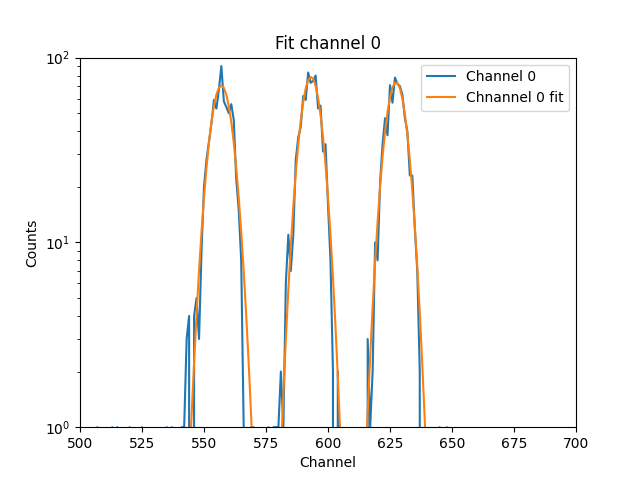
\includegraphics[scale = 0.6]{images/TT_21_Chn0.png}
    \captionof{figure}{Channel 0 spectrum fit with [\ref{eq:califit}]}
\end{center}

\begin{center}
    \label{TT_21}
    \centering
    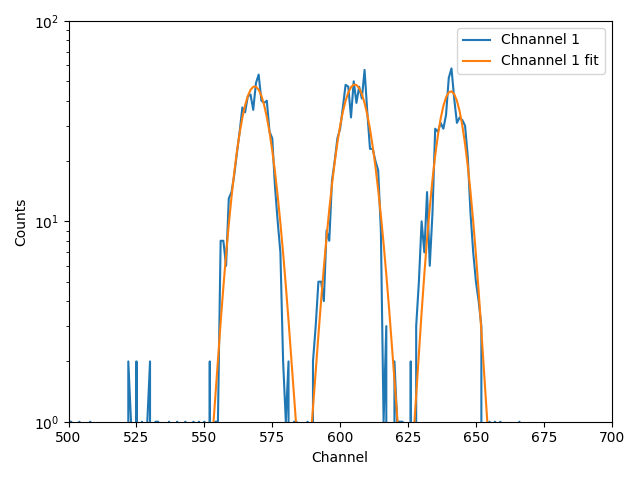
\includegraphics[scale = 0.6]{images/TT_21_Chn1.png}
    \captionof{figure}{Channel 1 spectrum fit with [\ref{eq:califit}]}
\end{center}

\begin{center}
    \label{TT_21}
    \centering
    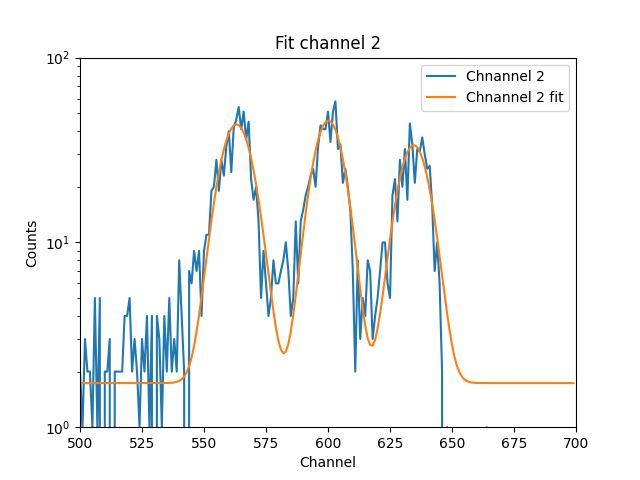
\includegraphics[scale = 0.6]{images/TT_21_Chn2.png}
    \captionof{figure}{Channel 2 spectrum fit with [\ref{eq:califit}]}
\end{center}

The fit parameters for means $\mu_0$, $\mu_1$ and $\mu_2$ in equation [\ref{eq:califit}] are the ones that represent the energy value of each peak in channels. The computed values for these parameters, as well as the theoretical values of the energy in MeV for the peaks, are organised in the following tables:

\begin{table}[H]
\centering
\begin{tabular}{|w{0.8cm}|w{3cm}|w{2cm}|}
\hline
Peak & Channel 0 [Chn] & Theoretical Energy [keV] \\ \hline
1\textsuperscript{st} & $ \mu_0 = 557.00 \pm 0.11 $ & 5156.59 \\ \hline
2\textsuperscript{nd} & $ \mu_1 = 593.14 \pm 0.10 $ & 5485.56 \\ \hline
3\textsuperscript{rd} & $ \mu_2 = 627.44 \pm 0.10 $ & 5804.82 \\ \hline
\end{tabular}
\caption{Calibration Values for Channel 0}
\label{tab:calibration0}
\end{table}

\begin{table}[H]
\centering
\begin{tabular}{|w{0.8cm}|w{3cm}|w{2cm}|}
\hline
Peak & Channel 1 [Chn] & Theoretical Energy [keV] \\ \hline
1\textsuperscript{st} & $ \mu_0 = 568.52 \pm 0.17 $ & 5156.59 \\ \hline
2\textsuperscript{nd} & $ \mu_1 = 605.39 \pm 0.17 $ & 5485.56 \\ \hline
3\textsuperscript{rd} & $ \mu_2 = 640.77 \pm 0.17 $ & 5804.82 \\ \hline
\end{tabular}
\caption{Calibration Values for Channel 1}
\label{tab:calibration1}
\end{table}

\begin{table}[H]
\centering
\begin{tabular}{|w{0.8cm}|w{3cm}|w{2cm}|}
\hline
Peak & Channel 2 [Chn] & Theoretical Energy [keV] \\ \hline
1\textsuperscript{st} & $ \mu_0 = 563.09 \pm 0.28 $ & 5156.59 \\ \hline
2\textsuperscript{nd} & $ \mu_1 = 600.15 \pm 0.26 $ & 5485.56 \\ \hline
3\textsuperscript{rd} & $ \mu_2 = 634.56 \pm 0.36 $ & 5804.82 \\ \hline
\end{tabular}
\caption{Calibration Values for Channel 2}
\label{tab:calibration2}
\end{table}

Using the values in these three tables we now need to compute a calibration equation for each of the channels.
We plotted the theoretical values of the energy of the three peaks as a function of fit parameters:

\begin{center}
    \label{TT_21}
    \centering
    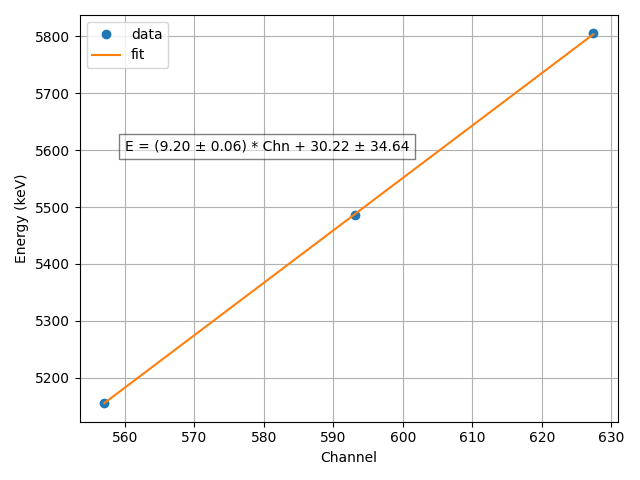
\includegraphics[scale = 0.6]{images/TT_21_Chn0_calib.png}
    \captionof{figure}{Calibration Channel 0}
\end{center}

The calibration equation for channel 0 is:

\begin{equation}
    \begin{split}
        E[\text{MeV}] &= m_0 \times E[\text{Chn}] + b_0 \\
        m_0 &= 9.20 \pm 0.06 \\
        b_0 &= 30.22 \pm 34.64
    \end{split}
    \label{eq:calib0}
\end{equation}

\begin{center}
    \label{TT_21}
    \centering
    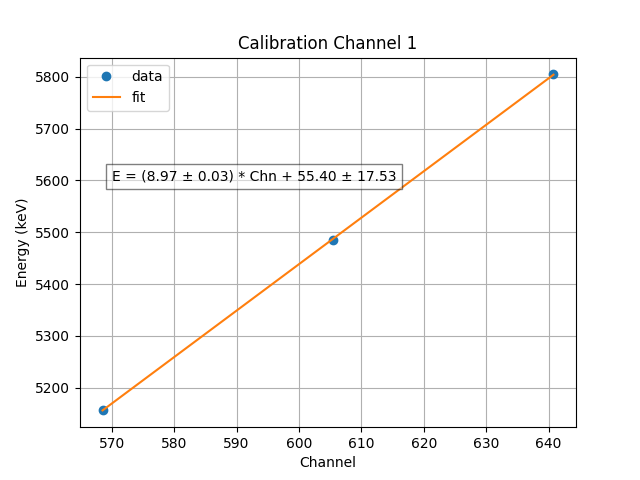
\includegraphics[scale = 0.6]{images/TT_21_Chn1_calib.png}
    \captionof{figure}{Calibration Channel 1}
\end{center}

The calibration equation for channel 1 is:

\begin{equation}
    \begin{split}
        E[\text{MeV}] &= m_1 \times E[\text{Chn}] + b_1 \\
        m_1 &= 8.97 \pm 0.03 \\
        b_1 &= 55.40 \pm 17.53
    \end{split}
    \label{eq:calib1}
\end{equation}

\begin{center}
    \label{TT_21}
    \centering
    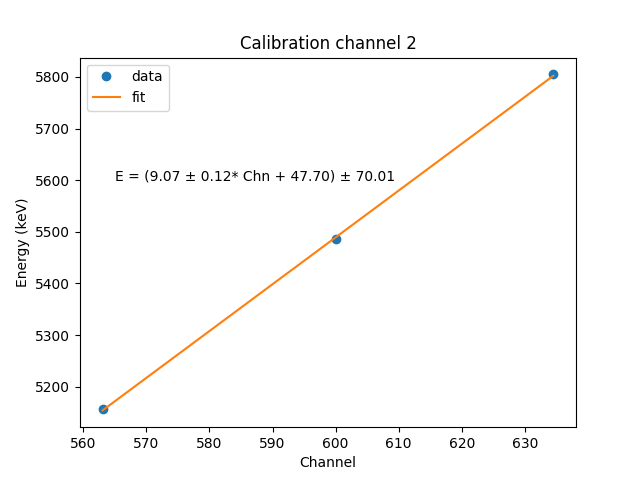
\includegraphics[scale = 0.6]{images/TT_21_Chn2_calib.png}
    \captionof{figure}{Calibration Channel 2}
\end{center}

The calibration equation for channel 2 is:

\begin{equation}
    \begin{split}
        E[\text{MeV}] &= m_2 \times E[\text{Chn}] + b_2 \\
        m_2 &= 9.07 \pm 0.12 \\
        b_2 &= 48.17 \pm 69.69
    \end{split}
    \label{eq:calib2}
\end{equation}

\section{ Lithium Fluoride Sample}

$\ce{LiF}$

\section{ Lithium Aluminate Sample}

$\ce{LiAlO_2}$

\subsection{Energy Profile}



\section{Implanted Sample}

\section{Conclusion}

\section{Perguntas}

\begin{enumerate}
    \item Para a calibração, colocamos os valores e as incertezas de todos os 10 parâmetros para cada channel ou apenas colocamos as médias ?
\end{enumerate}

\section{}


\printbibliography
\nocite{*}

\end{multicols}

\end{document}